\documentclass{scrreprt}
\usepackage[polish]{babel}
\usepackage[utf8]{inputenc}
\usepackage{listings}
\usepackage{graphicx}
\usepackage{aeguill}
\usepackage[bookmarks=true]{hyperref}
\hypersetup{
    bookmarks=false,    % show bookmarks bar?
    pdftitle={AGHydra - aimo},    % title
    pdfauthor={Yiannis Lazarides},                     % author
    pdfsubject={TeX and LaTeX},                        % subject of the document
    pdfkeywords={TeX, LaTeX, graphics, images}, % list of keywords
    colorlinks=true,       % false: boxed links; true: colored links
    linkcolor=blue,       % color of internal links
    citecolor=black,       % color of links to bibliography
    filecolor=black,        % color of file links
    urlcolor=purple,        % color of external links
}%
\def\myversion{1.0 }
\title{%
\flushright
\rule{16cm}{5pt}\vskip1cm
\Huge{Analiza\\ i Modelowanie Oprogramowania \\ - projekt}\\
\vspace{2cm}
dla\\
\vspace{2cm}
AGHydra System\\
\vspace{2cm}
Przygotowane przez:\\
Bartosz Śliwa\\
Michał Dziedzic\\
Daniel Poznański\\
\vfill
\rule{16cm}{5pt}
}
\date{}
\usepackage{hyperref}
\begin{document}
\maketitle
\tableofcontents
\chapter{Ogólny opis systemu}
\chapter{Analiza dziedziny}
\section{Definicje i skróty}
\chapter{SRS - Specyfikacja wymagań}
\chapter{Architektura systemu}
\chapter{Projekt oprogramowania}
\chapter{Projekt interfejsu użytkownika IRS}

\section{Ekrany zorientowane wokół Wiki}
\begin{center}
	\makebox[\textwidth]{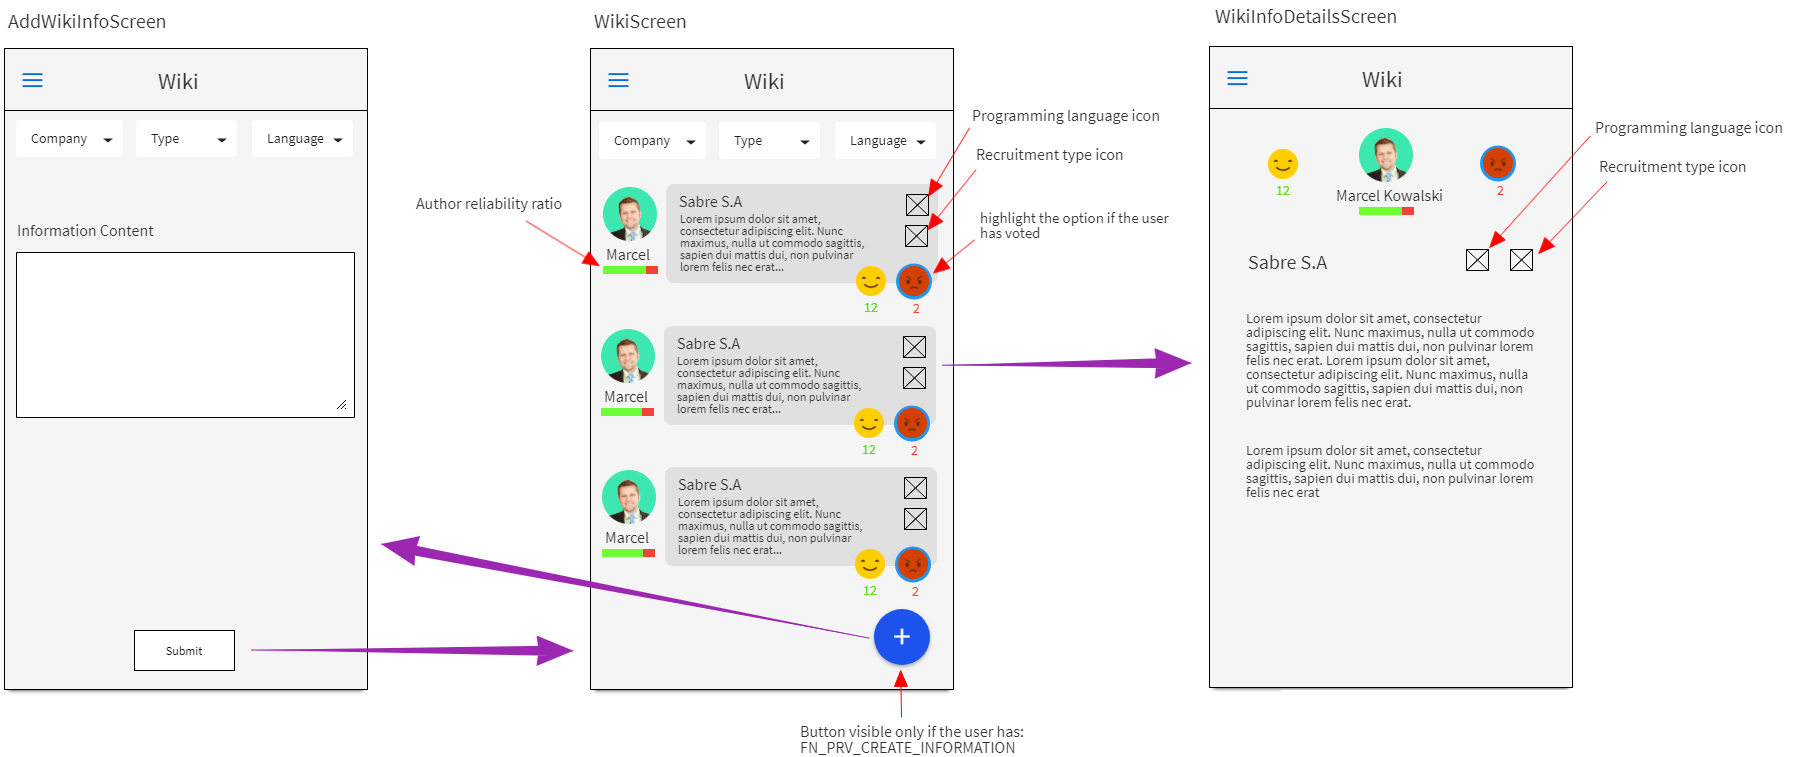
\includegraphics[width=\textwidth]{wiki_user_interface}}
\end{center}

\section{Ekrany zorientowane wokół Job i Referral}
\begin{center}
	\makebox[\textwidth]{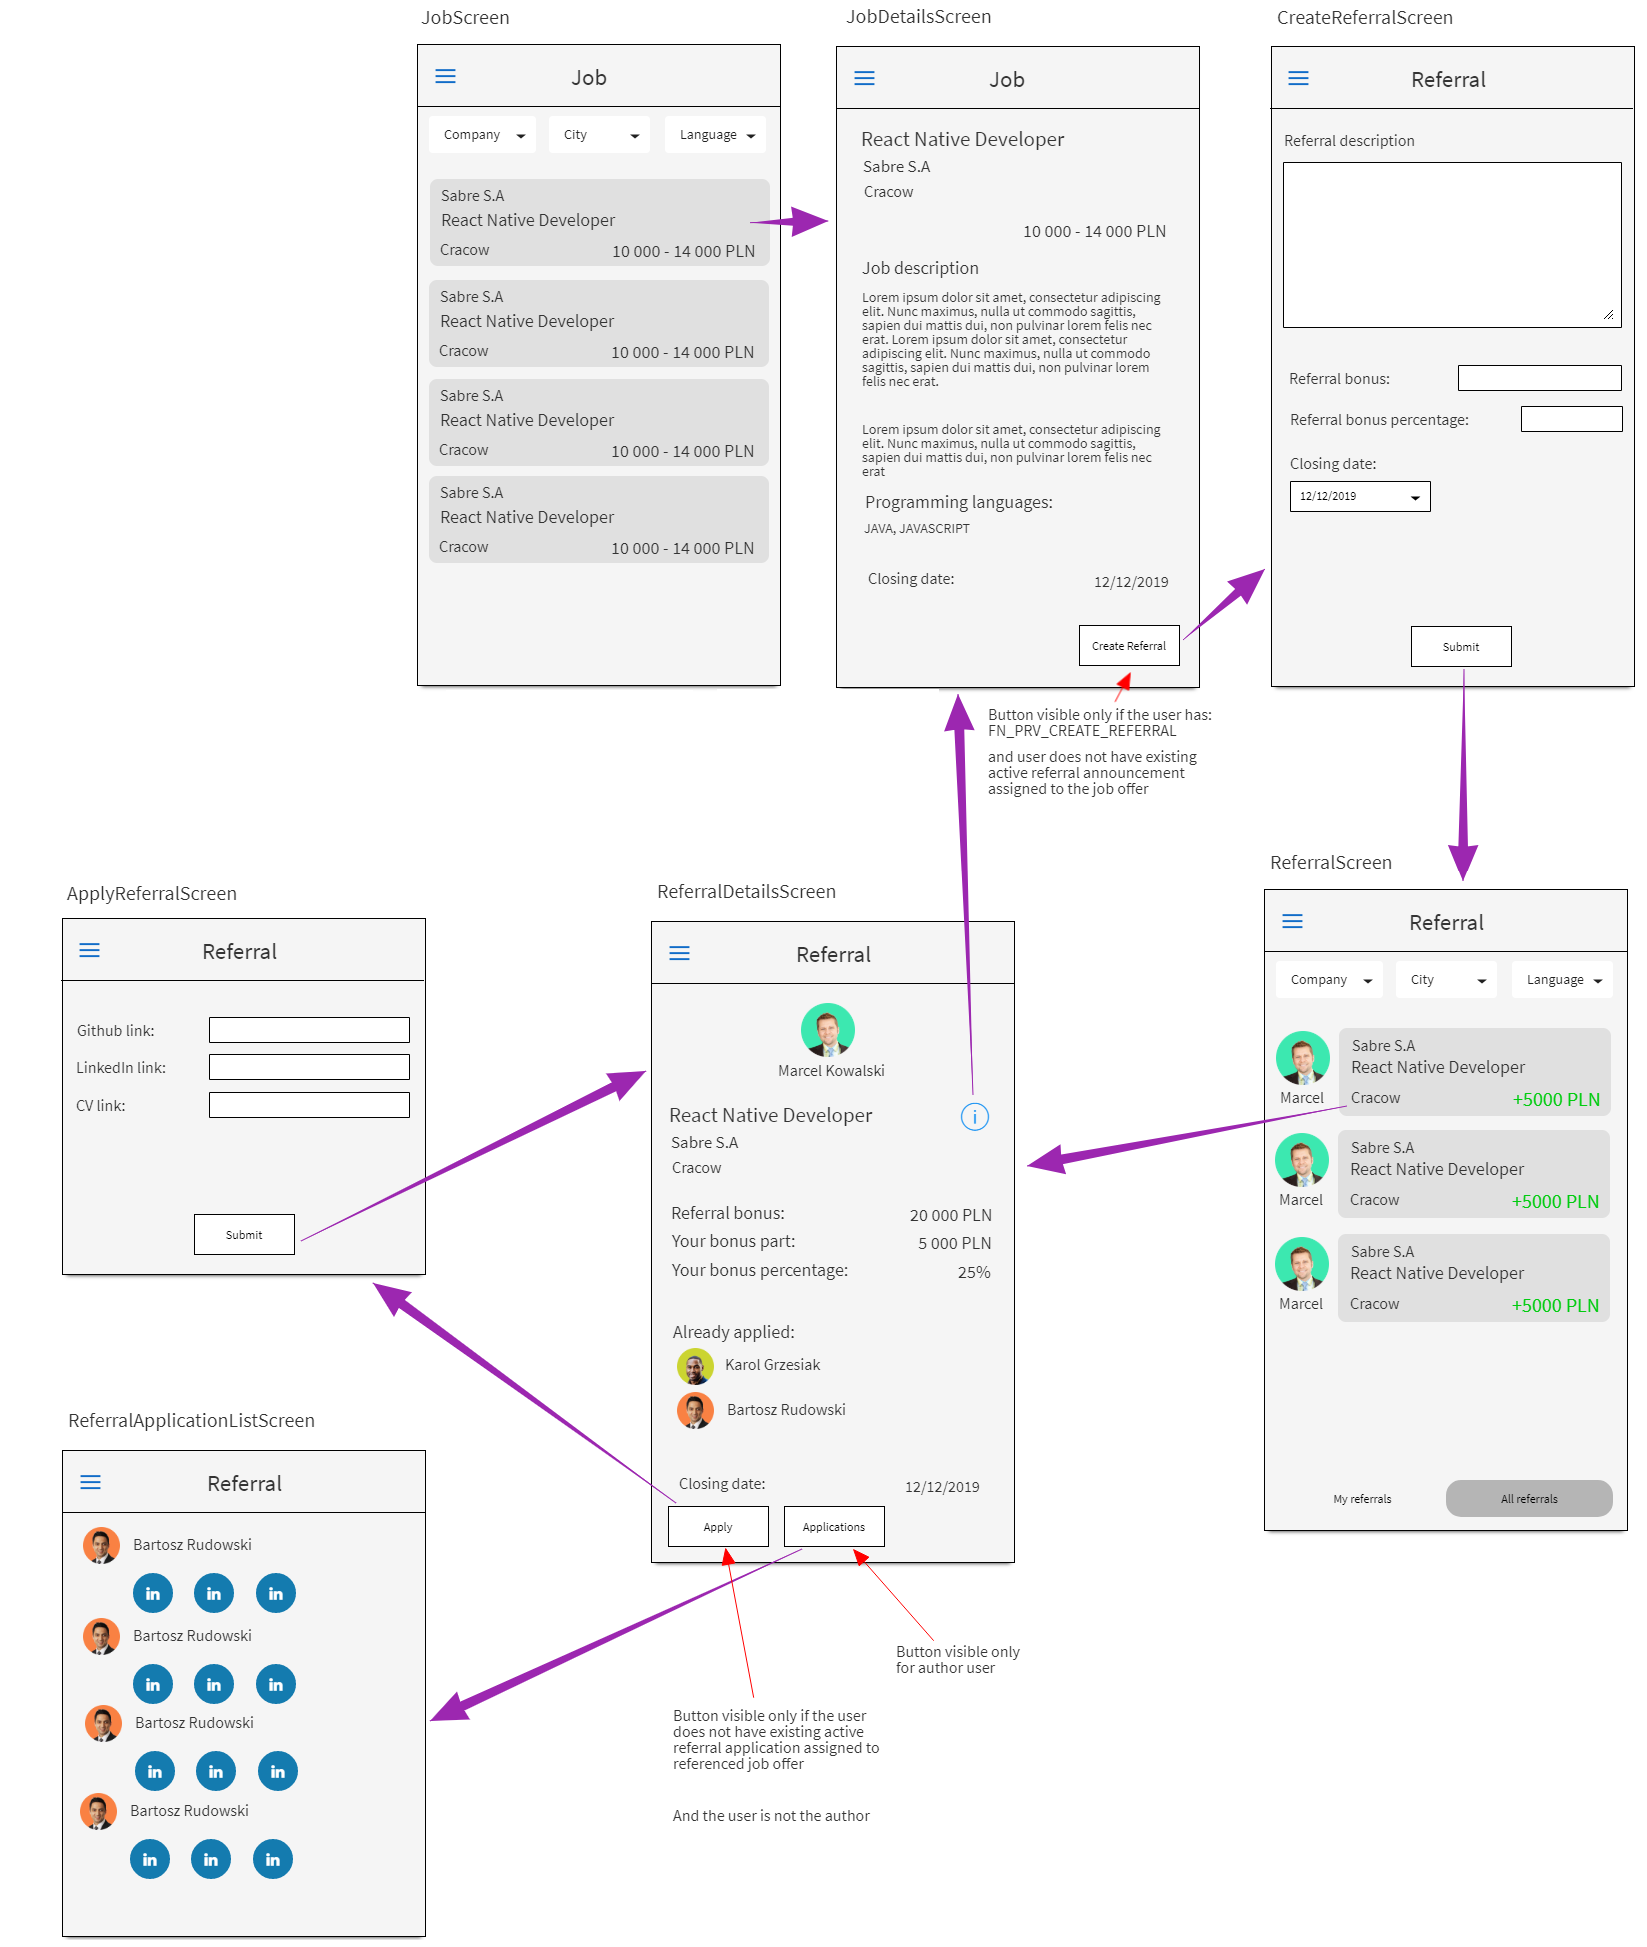
\includegraphics[width=\textwidth]{job_referral_user_interface}}
\end{center}


\chapter{Projekt bazy danych}

\section{Diagram ERD}
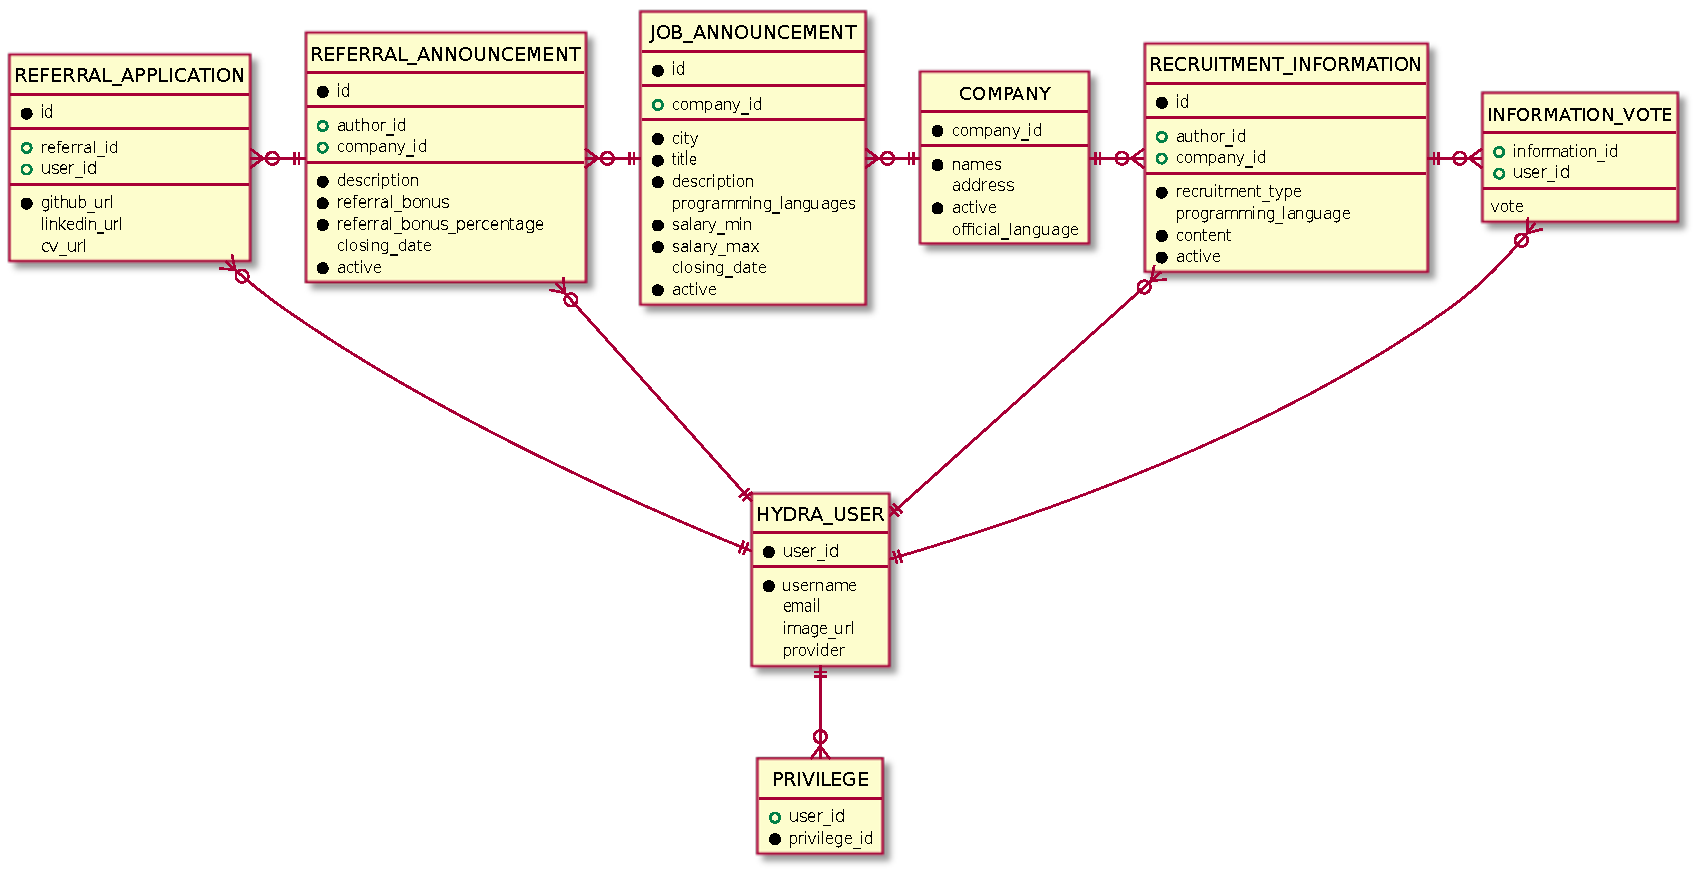
\includegraphics[width=\textwidth, keepaspectratio]{hydra_db_erd.pdf}

\section{Specyfikacja kwerend}


\end{document}